\chapter{Data acquisition and structure}

Before implementing and testing any group creation algorithms, we need to gather usable data
to perform testing on. The data consists of the topology size, and where in the topology a node is located.

For basic testing we can create our own data, and either assume the location of nodes, or randomly distribute them on a topology.

In a more reliable testing setup we should ideally get information from a real world data source. 
The topology would then represent a section of the world, being either a city, town or neighbourhood, and the nodes would be APs most likely located in each household.

\section{Requirements}
The testing data should be a set of nodes that has two coordinates $x$ and $y$ on a two-dimensional grid. Henceforth we will call refer to the populated grid as the topology. When the nodes are placed on the
topology, we can compute which nodes it can hear on the radio and add these to the node's SSID-scan list.
This list contains the names of all the nodes it can hear, and how loud it is heard measured in $-dBi$.
Additionally the following parameters should be variable depending on each test scenario:
\begin{itemize}
\item Topology size, variable width of x- and y-axis.
	\item Number of nodes
\item Minimum distance between nodes (in meters)
	\item Minimum loudness measured in $-dBi$ for a node to account another node as a neighbour (e.g -100 is too low for anyone to hear).
	\end{itemize}

	\section{Program design}
	The topology generation program consists of two main functionalitites.

	The first functionality is being  be able to create a topology and generate nodes which are uniformly
	and randomly positioned on the network topology. The size of the topology, the number of nodes and the minimum distance
	between nodes are properties that can be given as input arguments to the program. 

	The second functionality is computing which nodes can hear each other. We are assuming all nodes
	are transmitting with equal strength, and that the environment is flat and obstacle free. 
	All the neighbouring nodes that can be heard by a node, is added to its list of neighbours, and it stores the $-dBi$ value so it later can be shared with
	the group. 

	The resulting program, written in Python 3\cite{Python3}, contains an importable \textit{topology class}. This way, for further testing we can use different data sources to get the positions of nodes,
	and only let the topology class compute the list of neighbours. 

	The interference levels between APs is calculated by iterating through all the nodes. For each node $N$ we record its x and y position,
	and then start a second iteration through the nodes. For each node $n$ in the second iteration we calculate the distance $d$ in
	meters between $N$ and $n$ using Euclidean distance. Knowing the the distance between the nodes,  we can use the formula for free space path loss \cite{FSPL} to compute the $-dBI$ values. The code can be seen in figure \ref{fig:dbiCreation}.


	For the sake of cross compatibility with other applications, the result of the computation represented in json. A topology consists of as many JSON node-objects as there are nodes.

	\begin{figure}[H]
	\begin{python}
#In topology class
def measureInterference(self):
 for nodeSubject in self._nodes:  
  for nodeObject in self._nodes:
    nodeSubject.calculateInterferenceTo(nodeObject) 

#In node class
def calculateInterferenceTo(self, nodeObject):
 if self == nodeObject:
  return
 dist = round(self.distanceTo(nodeObject))

#If  nodes have same coordinate, set high interference. 
 if (dist == 0):
  dBi = -40
 else:
  dBi  = self.measureDbi(dist) * -1

def measureDbi(self, dist):
 return (20 * math.log(self._frequency, 10)) + 
(20 * math.log(dist, 10)) - 27.55

			\end{python}
			\caption{Computing the interference between nodes}
			\label{fig:dbiCreation}
			\end{figure}
			\section{Data output and visual representation} \label{simulationrep}
			Figure following illustrates the node structure, and is an example of how a node with two neighbours will look: 
			\begin{figure}[H]
			\begin{minipage}{\linewidth}
			\begin{lstlisting}[language=json]
1: {
 "posX": 100,
 "posY": 100, 
 "ssid": "NODE1",
 "neighbourCount": 2, 
 "neighbours": {
    0: {
     "ssid": NODE2,
     "dbi": -77.23
    },
    1: {
     "ssid": NODE3,
     "dbi": -79.52
    }
  }
}
\end{lstlisting}
\end{minipage}
\caption{JSON output structure}
\label{fig:nodeStruct}

\end{figure}
We can run the program in the following way
\begin{verbatim}./GenerateTopology.py -n 200 -w 100 -h 100 --space 10 --dbi 85 \end{verbatim}
Which instructs the program to create a topology with 200 nodes. 
The topology should be 100 by 100 meters large, and there should be at least 10 meters
between each node. The $dbi$ parameter makes sure that only nodes which can be
heard with a $-dBi$-value of $-85$ or larger should be considered neighbours.

The output is a 3.8 MB large file containing the resulting topology-data in JSON.

By writing a simple JavaScript browser application meant to interpret the output, we can
visually represent the nodes on a grid, and the result will look like what can be seen in figure \ref{fig:randtop}

\begin{figure}
\center
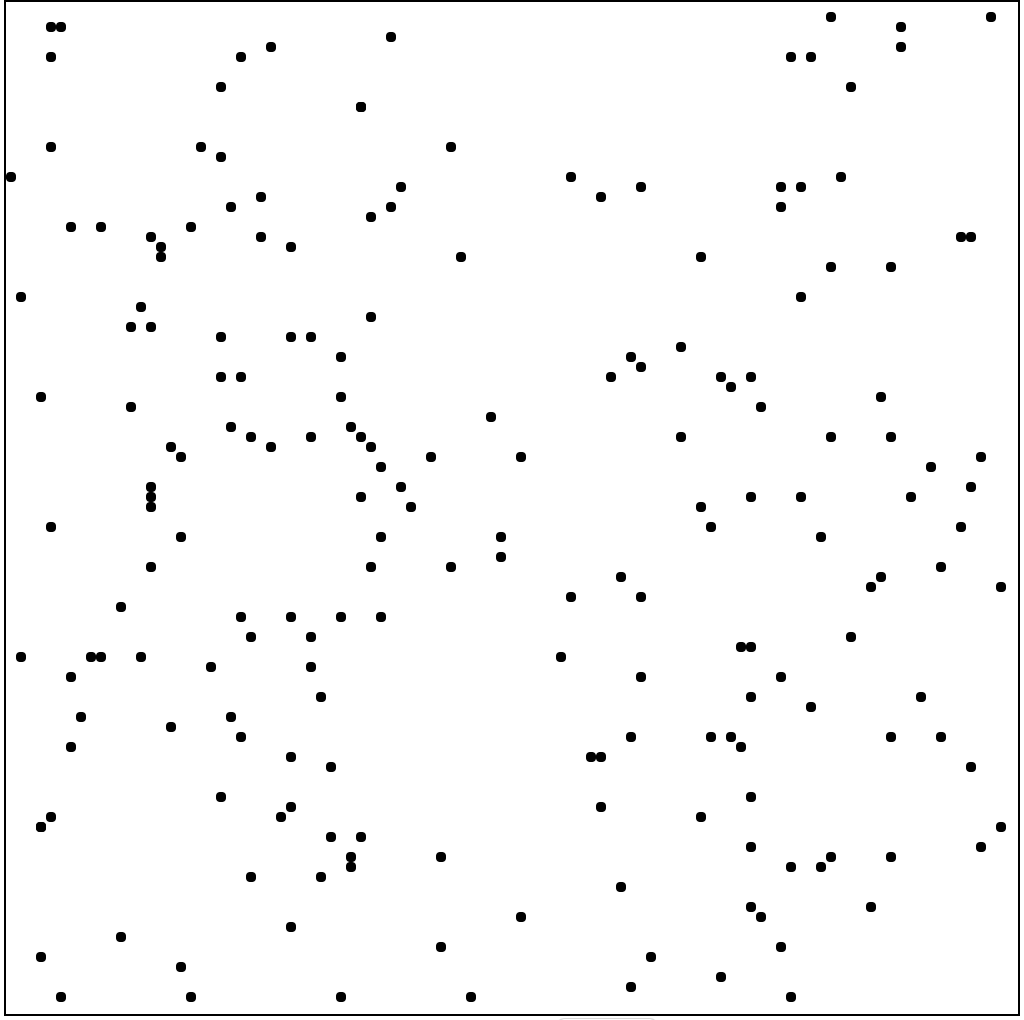
\includegraphics[scale=0.4]{Images/randomtopology.png}
\caption{Generated topology with random, uniform distribution}
\label{fig:randtop}
\end{figure}

\section{WiGLE}
WiGLE (Wireless Geographical Logging Engine) \cite{wigle} is a project started in 2001
which purpose is to gather information about wireless networks. The data they have
accumulated in their database is entirely user submitted. Anyone can download an 
Android app  published by WiGLE, and then use the app for wardriving
\footnote{Wardriving is the act of tracking wireless networks using a laptop or a phone,
	and then store the information about each network \cite{Wardriving}.},
	then submit the data to WiGLE's centralized database. All the APs can be viewed on an interactive
	map provided on WiGLE's website. The data can also be accessed through an API call.
	Using their service is entirely free, but the amount of data
	that can be requested is throttled on a day-to-day basis. As they openly support
	research projects, they provided us with an account with a slightly higher daily data
	limit.

	To us this is interesting because we can use the location of APs to
	create more realistic network topologies, and see how well the algorithm 
	performs on these. 


	\subsection{REST API}
	Their REST API provides data presented in JSON, and offers different services,
	such as user profile operations, statistical information and network search.

	We only need to use the networks search part of the API for our purpose. 
	By passing it a request for nodes between two latitudes
	and longitudes, the API responds with the APs in that area.  
	A request will look something like what can be seen in figure \ref{fig:wigReq}
	\begin{figure}
	\begin{lstlisting}[breaklines]
	https://api.wigle.net/api/v2/network/search?first=0&latrange1=37.808469&latrange2=37.746744&longrange1=-122.539232&longrange2=-122.381355
	\end{lstlisting}
	\caption{Example of a Wigle API request}
	\label{fig:wigReq}
	\end{figure}
	The parameters $latrange1$ and $longrange1$ are the coordinates that marks the beginning 
	of the area we are interested in, where $latrange2$ and $longrange2$ marks the end. 
	As WiGLE at most returns information about 100 APs for every query, we need the $start$
	parameter to tell WiGLE at which index offset we want to begin fetching data from.
	A start value of $0$ means we fetch in the range $0-99$, a value of $100$ means in the
	range $100-199$ and so on. The JSON response for a succesful request for an AP,
	can be seen in figure \ref{fig:wigle}.

	\begin{figure}

	\begin{lstlisting}[language=json]
{
	"userfound": false,
		"qos": 0,
		"comment": null,
		"lastupdt": "2015-12-22T17:49:34.000Z",
		"bcninterval": 0,
		"dhcp": "?",
		"lasttime": "2015-12-22T17:49:15.000Z",
		"trilong": 10.82792618,
		"netid": "5C:9E:FF:2B:54:84",
		"freenet": "?",
		"trilat": 62.2816925,
		"name": null,
		"firsttime": "2015-12-22T20:55:01.000Z",
		"type": "infra",
		"ssid": "NETGEAR23",
		"paynet": "?",
		"wep": "2",
		"transid": "20151222-00207",
		"channel": 52
}

\end{lstlisting}
\caption{REST API response with AP data}
\label{fig:wigle}
\end{figure}

We are primarily interested in the properties $trilong$ and $trilat$, which is
the triangulated coordinates of the AP. 

\subsection{Using Wigle data}
WiGLE provides data about the location of access points. However, to be able to
use the data for our group computation, we must translate the global coordinates
to two dimensional coordinates. We can then place each AP on a topology with the
same format as the generated topologies we created in section \ref{simdata}.
This is necessary for two reasons.

The first reason is that creating a group creation program that can operate
on the longitudes and latitudes directly adds more complexity. Both with regards to
group computation and visual representation. 

The second reason is that the WiGLE data does not contain information about
which neighbours each AP can hear, and with what $-dBi$ strengths they are heard.
This will have to be computed like earlier, and by parsing it to the format
we designed in section \ref{simulationrep} we can reuse the code to generate the neighbour lists.

The haversine formula [[ref or explain]] gives us the distance in meters between two coordinates. By calculating
the distane between the latitude startpoint and the latitude endpoint, we can get the size of one
axis in meters. By computing the distance between the longitude start and endpoint we get the size of the
other axis. To place a node correctly in the coordinate system, we simply use the haversine formula on the
origin coordinates to compute the distances between each axis. 

All of this has been implemented in a python program. As input it takes both latitude and longitude start and end coordinates,
    then fetches all nodes within that range and inserts them on a plane. 


